\section{Krabička pro nástěnný snímač prostorové teploty}
\label{sec:krabicka-pro-nastenny-snimac-prostorove-teploty}
Krabička pro nástěnný snímač prostorové teploty je vytisknuta na 3D tiskárně Prusa i3 MK3s MMU2s (čelní strana je na obrázku \ref{fig:krabicka-nastenny-snimac-prostorove-teploty-predni-strana}). Použitý plast je \acrshort{pet-g} (\textit{\acrlong{pet-g}}), bílá barva byla požadovaná uživatelem. Výhody zejména tohoto materiálu jsou houževnatost, pevnost a dobré propojování vrstev při tisku. Návrh modelu jsem provedl v softwaru FreeCAD. Samotnou přípravu modelu pro tisk jsem provedl v~PrusaSliceru. Krabička má rozměry 130 × 99 × 26 mm a skládá ze dvou dílů. Krabička jak pro verzi s Ethernetem, tak i pro WiFi je stejná, liší se jen konektorem pro RJ45 a DC konektorem pro adaptér.

Spodní díl slouží k uchycení DPS, která je umístěná na distančních sloupkách (dochází tak k lépe odvádění tepla ze součástek). Spodní díl má v horní části průduchy na odvětrávání tepla. Ve spodní části je vymezená oblast s~průduchy pro teplotní senzor, který se nachází nad nimi. Dále je tato oblast ohraničená přepážkou, aby nedocházelo přílišnému míchání vzduchu z prostoru DPS a teplotního čidla. Na obvodu se nacházejí sloupky pro uchycení horní části krabičky. Distanční sloupky i sloupky pro horní části obsahují v~otvoru závitovou vložku (tepelně vložená do otvoru), dochází tak optimální přidělání dílů za pomocí metrického šroubku (nedochází k pnutí a možnému prasknutí jako v případě, pokud by se použil samovrtný šroubek). Dále se na spodním dílu nacházejí čtyři díry pro uchycení na zeď, v jejich oblasti je plast ještě zesílen. Na druhé straně spodního dílu jsou distanční sloupky, které slouží k~tomu, aby při přivrtání ke zdi, krabička neležela přímo na zdi, ale aby pod ní docházelo k odvětrávání horní části krabičky a k proudění vzduchu ve spodní části v oblasti teplotního čidla.

Horní část krabičky obsahuje otvory pro displej a tlačítka. Na čelní straně se nacházejí uprostřed průduchy pro teplotní senzor, dále uvnitř této oblasti je vytvořená přepážka, která dosedá na spodní část přepážky spodního dílů, tato vzduchová kapsa je tedy oddělená od zbytku krabičky, aby teplotní senzor nebyl ovlivněn moc teplotou samotné krabičky. Dále se na čelní straně nacházejí průchody pro konektor RJ45 pro variantu s Ethernetem nebo průchod pro DC napájecí konektor, dále průchod pro konektor UARTu. Horní část je přichycena ke spodní čtyřmi šroubky, jejichž hlavičky jsou utopené a~nepřečnívají na povrchu.

Jednotlivé díly jsou zobrazeny v příloze \ref{app:krabicka-pro-nastenny-snimac-prostorove-teploty}, dále jsou zde fotografie části krabičky s umístěnou DPS. Krabička je poměrně robustní, spodní tlouštka stěny je 2 mm, obvodové stěny jsou též 3 mm silné a čelní strana má 2 mm. Samotné uchycení na stěnu je velmi stabilní. U verze s Ethernetem je chyba v návrhu v DPS, spočívající nedostatečném vysunutí konektorů z DPS, což je vidět, že konektory nejsou zarovnané s čelní stranou krabičky, nicméně na funkčnost používaní konektorů to nemá vliv. Ve verzi s WiFi je tato chyba opravena. Hmatníky na tlačítka nejsou vytisknuté, ty byly zakoupeny.
 
\begin{figure}[H]
    \centering
    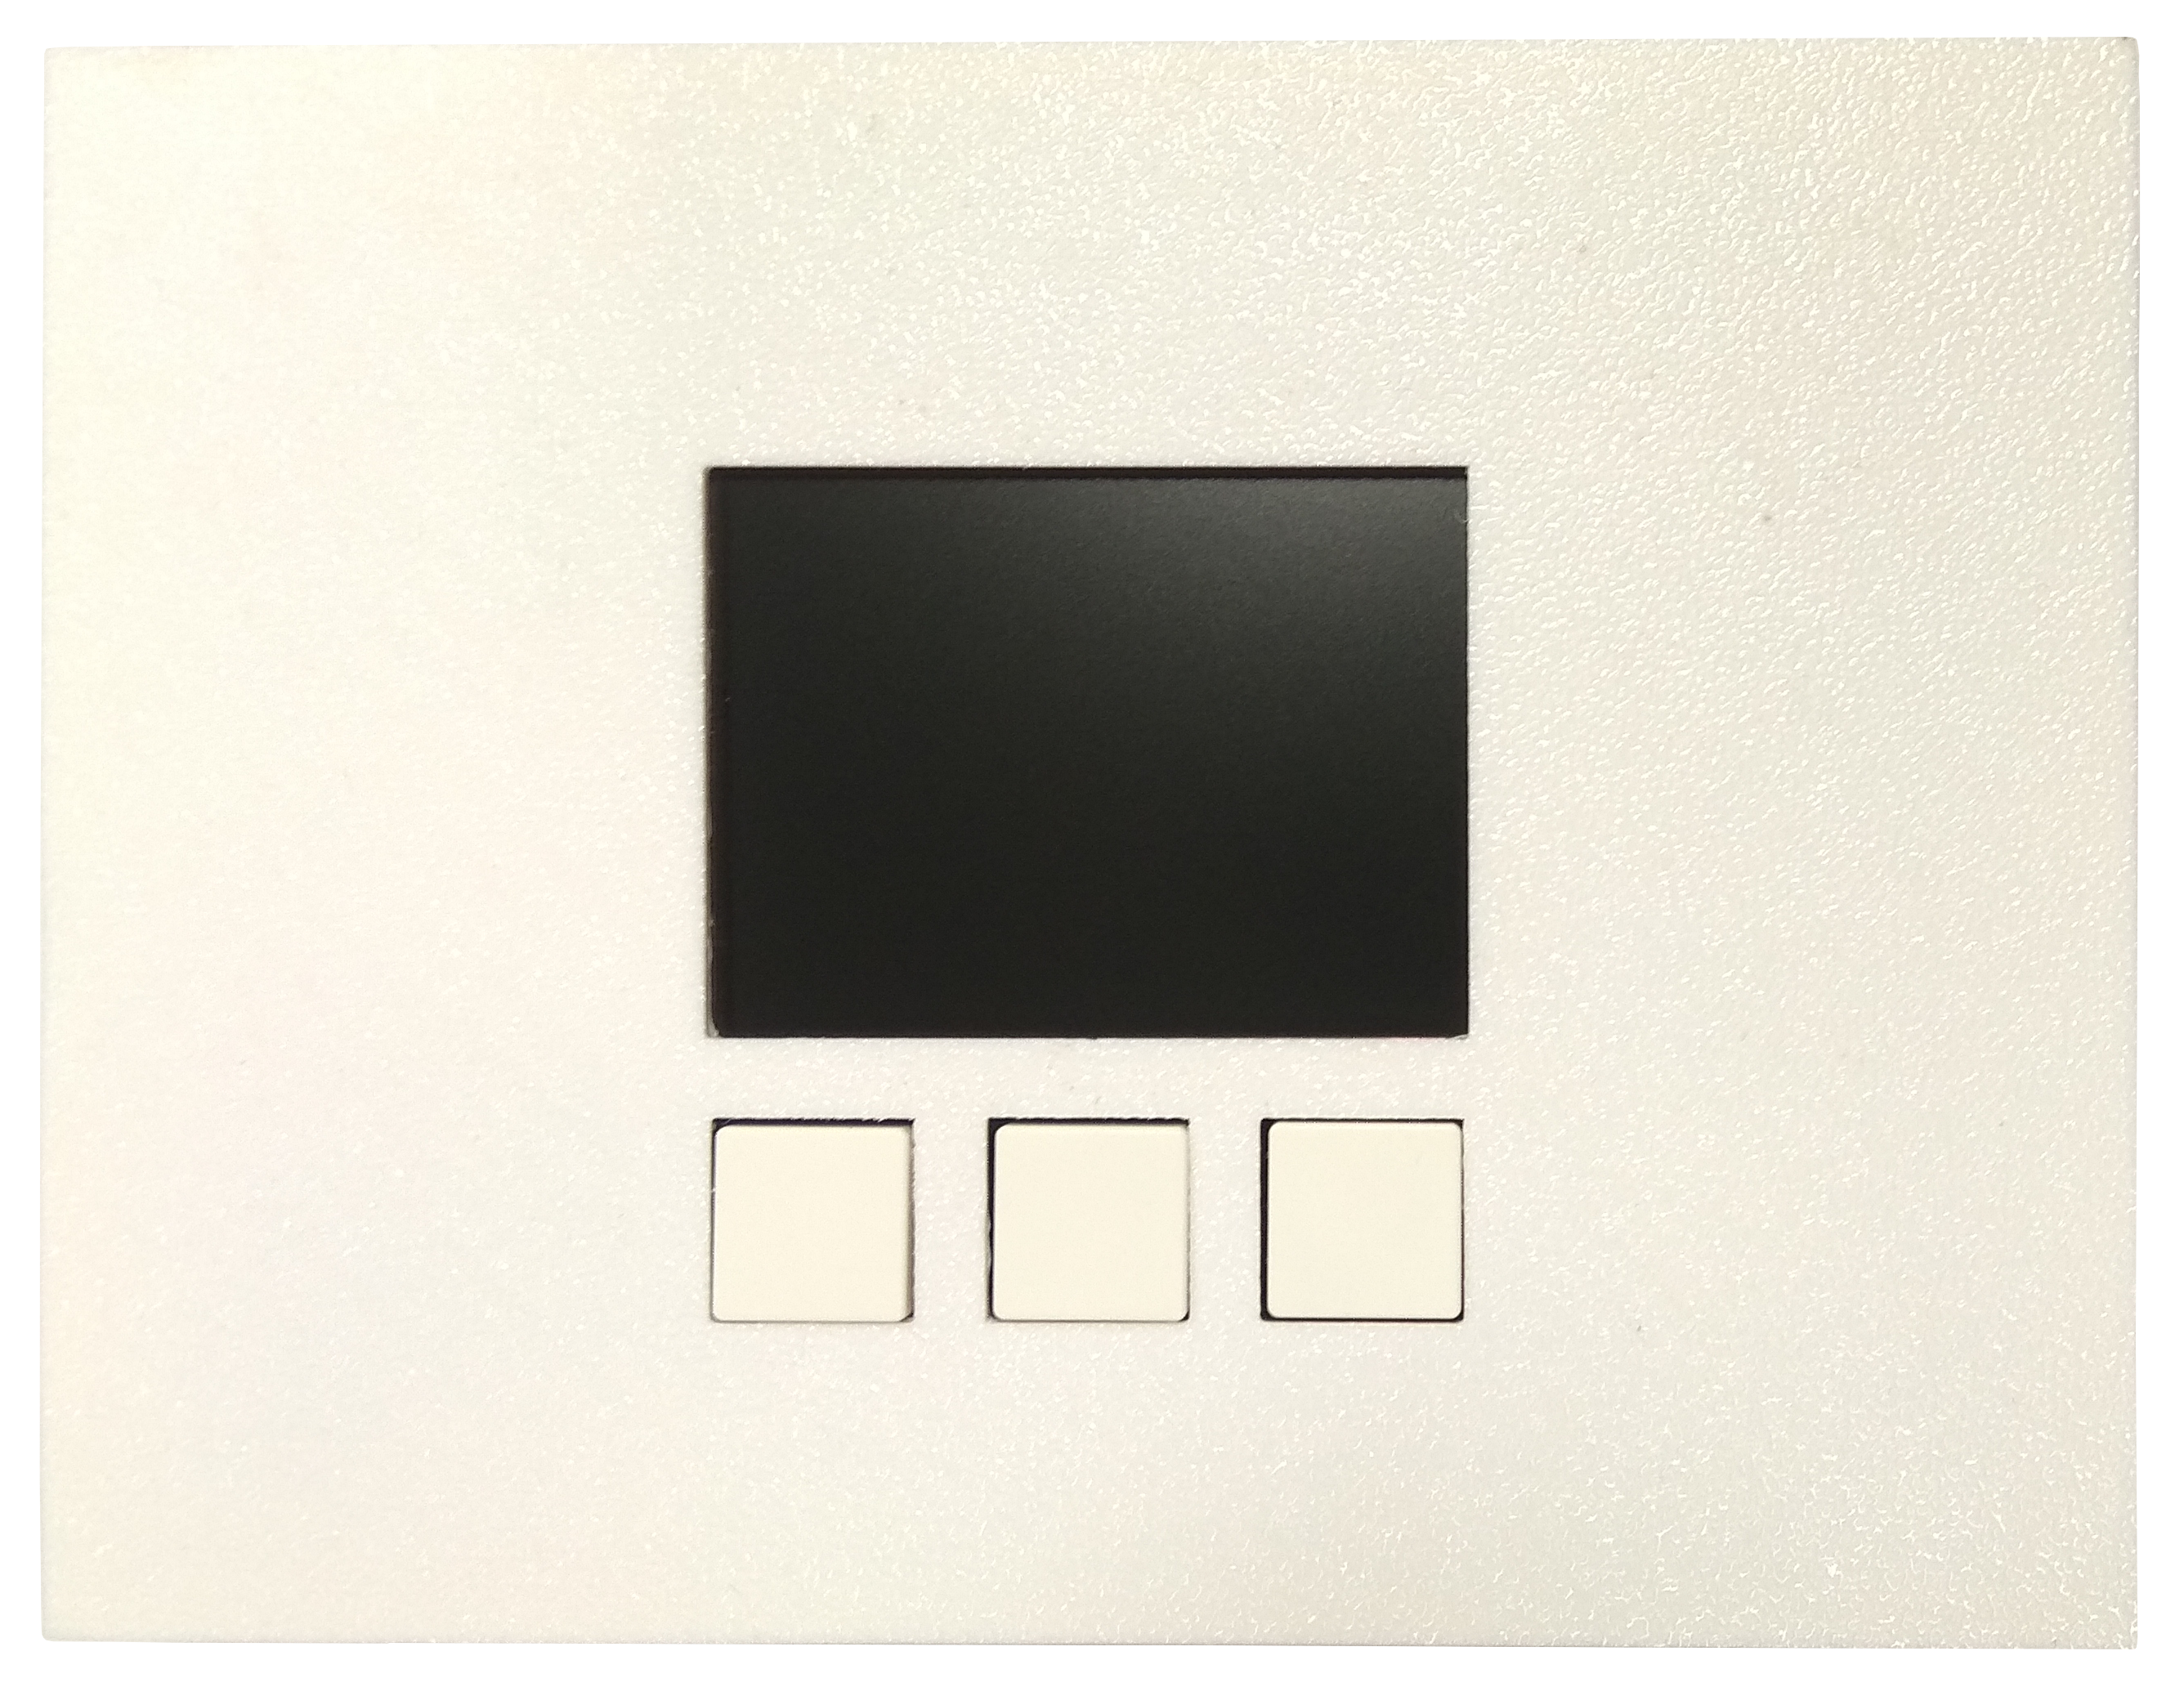
\includegraphics[width=0.89\textwidth]{images/krabicka-nastenny-snimac-prostorove-teploty/krabicka-nastenny-snimac-prostorove-teploty-predni-strana-displej.png}
   \caption{Čelní strana krabičky.}
    \label{fig:krabicka-nastenny-snimac-prostorove-teploty-predni-strana-displej}
\end{figure}
